\documentclass[12pt,a4paper]{article}

% ─── 1. PACKAGES ──────────────────────────────────────────────────────────────
\usepackage[utf8]{inputenc}
\usepackage[T1]{fontenc}
\usepackage{amsmath, amssymb}
\usepackage{geometry}
\usepackage{graphicx}
\usepackage{xcolor}
\usepackage{listings}
\usepackage{hyperref}
\usepackage{booktabs}
\usepackage{enumitem}
\usepackage{tcolorbox}
\usepackage{mdframed}
\usepackage{fancyhdr}
\usepackage{titlesec}
\usepackage{tikz} 
% Menambahkan 'decorations.pathreplacing' untuk memperbaiki error pada brace
\usetikzlibrary{shapes.geometric, positioning, arrows.meta, calc, decorations.pathreplacing}

% Font Settings
\usepackage{newtxtext,newtxmath} % Times New Roman
\usepackage{courier}             % Courier New untuk kode

\geometry{margin=2.5cm}

% ─── 2. WARNA TEMA ────────────────────────────────────────────────────────────
\definecolor{codebg}{RGB}{245,247,250}
\definecolor{codeframe}{RGB}{180,195,215}
\definecolor{keywordcolor}{RGB}{0,112,192}
\definecolor{commentcolor}{RGB}{100,160,100}
\definecolor{stringcolor}{RGB}{180,70,50}
\definecolor{notebg}{RGB}{255,249,230}
\definecolor{noteframe}{RGB}{230,180,50}
\definecolor{tipbg}{RGB}{230,245,235}
\definecolor{tipframe}{RGB}{50,160,90}
\definecolor{sectioncolor}{RGB}{30,80,150}

% ─── 3. STYLE SECTION & TOC ───────────────────────────────────────────────────
\titleformat{\section}{\Large\bfseries\color{sectioncolor}}{}{0em}{\thesection\quad}[\titlerule]
\titleformat{\subsection}{\large\bfseries\color{sectioncolor!80}}{}{0em}{\thesubsection\quad}

% Style Table of Contents
\usepackage{tocloft}
\renewcommand{\cftsecleader}{\cftdotfill{\cftdotsep}}
\renewcommand{\cftsecfont}{\bfseries\color{sectioncolor}}

% ─── 4. LISTINGS (CODE STYLE) ─────────────────────────────────────────────────
\lstdefinestyle{customstyle}{
  basicstyle=\ttfamily\small,
  backgroundcolor=\color{codebg},
  frame=single,
  rulecolor=\color{codeframe},
  keywordstyle=\bfseries\color{keywordcolor},
  commentstyle=\itshape\color{commentcolor},
  stringstyle=\color{stringcolor},
  numbers=left,
  numberstyle=\tiny\color{gray},
  breaklines=true,
  tabsize=4,
  showstringspaces=false
}
\lstset{style=customstyle}

% ─── 5. KOTAK CATATAN (MD-FRAME) ──────────────────────────────────────────────
\newmdenv[
  backgroundcolor=notebg, linecolor=noteframe, linewidth=2pt,
  leftline=true, topline=false, rightline=false, bottomline=false,
  innerleftmargin=10pt, innertopmargin=6pt, innerbottommargin=6pt, skipabove=8pt
]{notebox}

\newmdenv[
  backgroundcolor=tipbg, linecolor=tipframe, linewidth=2pt,
  leftline=true, topline=false, rightline=false, bottomline=false,
  innerleftmargin=10pt, innertopmargin=6pt, innerbottommargin=6pt, skipabove=8pt
]{tipbox}

% ─── 6. HEADER & FOOTER ───────────────────────────────────────────────────────
\pagestyle{fancy}
\fancyhf{}
\fancyhead[L]{\small\textit{Metodologi Penelitian}}
\fancyhead[R]{\small\textit{noteify -- Pendahuluan}}
\fancyfoot[C]{\thepage}
\renewcommand{\headrulewidth}{0.4pt}

% ─── 7. DATA COVER ────────────────────────────────────────────────────────────
\title{
  {\LARGE\bfseries METODOLOGI PENELITIAN}\\[0.5em]
  {\large Modul Pembelajaran: Pengantar dan Konsep Dasar Sains}\\[0.8em]
  {\normalsize Penjelasan menyeluruh mengenai hakikat ilmu, penalaran logis, klasifikasi pendekatan, serta siklus tahapan penelitian ilmiah.}
}
\author{}
\date{}

% ==============================================================================
\begin{document}

\maketitle
\thispagestyle{fancy}
\tableofcontents
\newpage

% ─── KONTEN MATERI ─────────────────────────────────────────────────────────────

\section{Hakikat Ilmu Pengetahuan (Sains)}

\subsection{Apa itu Sains?}
Sebelum kita melangkah jauh ke metode penelitian, kita harus paham dulu apa itu "Sains" atau ilmu pengetahuan. Sains bukanlah sekadar kumpulan rumus atau hafalan, melainkan sebuah proses observasi sistematis terhadap peristiwa dan kondisi alam. Tujuannya adalah untuk menemukan fakta, merumuskan hukum, dan menyusun prinsip berdasarkan fakta-fakta tersebut.

Sains juga bisa diartikan sebagai kumpulan pengetahuan yang terorganisir, yang diperoleh dari hasil observasi, dan \textbf{dapat diverifikasi atau diuji ulang} melalui penyelidikan lebih lanjut. Kalau suatu pengetahuan nggak bisa diuji, maka itu belum bisa disebut sebagai sains.

\subsection{Fungsi dari Ilmu Pengetahuan}
Buat apa sih kita capek-capek meneliti dan mengembangkan ilmu? Sains punya tiga fungsi utama di kehidupan kita:
\begin{itemize}
    \item \textbf{Menjelaskan Kejadian (What):} Membantu kita memahami faktor-faktor apa saja yang menyebabkan sebuah fenomena itu bisa terjadi.
    \item \textbf{Menjelaskan Alasan (Why):} Mengungkap alasan mendasar di balik terjadinya suatu fenomena tersebut.
    \item \textbf{Memprediksi (Predict):} Ini yang paling canggih. Ilmu bisa memprediksi kemungkinan terjadinya suatu fenomena di masa depan, asalkan kondisi-kondisi tertentunya terpenuhi.
\end{itemize}

\subsection{Cara Manusia Memperoleh Pengetahuan}
Dalam kehidupan sehari-hari, sebelum pakai metode ilmiah yang ketat, manusia pada dasarnya mencari tahu sesuatu lewat dua cara mendasar:
\begin{enumerate}
    \item \textbf{Pengalaman (Experience):} Belajar dari apa yang kita alami sendiri. Contoh simpelnya: kita nggak sengaja menyentuh panci panas, lalu dari situ kita belajar dan tahu kalau benda panas itu bisa melukai kulit. Atau belajar mencari rute berkendara tercepat demi menghemat waktu dari pengalaman nyasar sebelumnya.
    \item \textbf{Otoritas (Authority):} Belajar dengan cara mempercayai sumber yang dianggap ahli atau punya otoritas. Misalnya kita dapet pengetahuan dari orang tua, guru, buku, atau koran. Contoh praktisnya: kita nanya ke sopir taksi yang udah puluhan tahun narik soal rute tercepat ngehindarin macet di dalam kota.
\end{enumerate}

\newpage
\section{Logika Penalaran dan Metode Ilmiah}

\subsection{Penalaran Induktif vs Deduktif}
Metode ilmiah itu sangat bergantung pada jalan pikiran kita. Ada dua mode penalaran yang jadi mesin penggerak penelitian:
\begin{itemize}
    \item \textbf{Penalaran Induktif (Dari Spesifik ke Umum):} Proses membuat generalisasi atau kesimpulan luas yang didasarkan dari beberapa observasi kecil. 
    \begin{itemize}
        \item \textit{Contoh:} Dosen ngecek lima buku metode penelitian yang berbeda, dan semuanya punya bab tentang "Sampel". Dosen itu lalu menyimpulkan (generalisasi): "Oh, berarti \textbf{semua} buku metode penelitian pasti punya bab sampel".
    \end{itemize}
    \item \textbf{Penalaran Deduktif (Dari Umum ke Spesifik):} Proses menarik kesimpulan khusus yang didasarkan pada prinsip, aturan umum, atau teori yang udah ada sebelumnya.
    \begin{itemize}
        \item \textit{Contoh:} Prinsip umumnya adalah "Semua atlet adalah siswa yang baik". Lalu kita punya fakta spesifik: "Adi adalah seorang atlet". Maka kesimpulan deduktifnya: "Adi pasti siswa yang baik".
    \end{itemize}
\end{itemize}

\subsection{Metode Hypothetico-Deductive}
Metode ilmiah yang paling umum dan sering dipakai di seluruh dunia adalah \textit{Hypothetico-Deductive Method}. Metode ini menggabungkan kekuatan induktif dan deduktif sekaligus!

\begin{figure}[h]
    \centering
    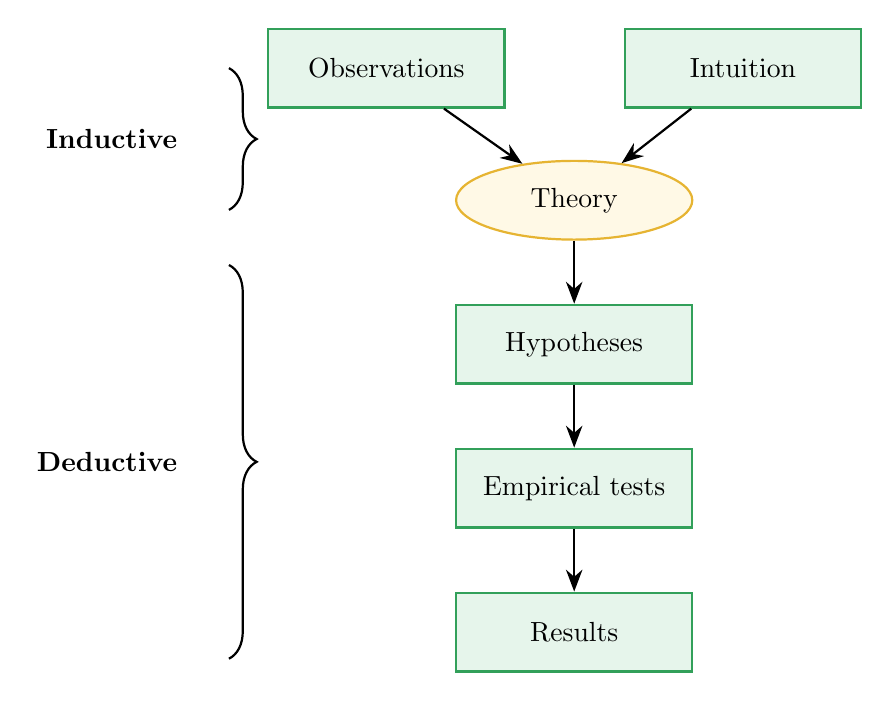
\begin{tikzpicture}[
        box/.style={draw, rectangle, minimum width=3cm, minimum height=1cm, align=center, fill=tipbg, draw=tipframe, thick},
        oval/.style={draw, ellipse, minimum width=3cm, minimum height=1cm, align=center, fill=notebg, draw=noteframe, thick},
        arr/.style={-{Stealth[scale=1.2]}, thick}
    ]
    
    % Inductive Part
    \node[box] (obs) {Observations};
    \node[box] (int) [right=1.5cm of obs] {Intuition};
    \node[oval] (theory) [below right=0.8cm and -0.2cm of obs] {Theory};
    
    % Deductive Part
    \node[box] (hyp) [below=0.8cm of theory] {Hypotheses};
    \node[box] (test) [below=0.8cm of hyp] {Empirical tests};
    \node[box] (res) [below=0.8cm of test] {Results};
    
    % Grouping braces
    \draw [decorate, decoration={brace, amplitude=10pt}, thick] (-2, 0) -- (-2, -1.8) node [midway, left=15pt] {\textbf{Inductive}};
    \draw [decorate, decoration={brace, amplitude=10pt}, thick] (-2, -2.5) -- (-2, -7.5) node [midway, left=15pt] {\textbf{Deductive}};
    
    % Arrows
    \draw[arr] (obs) -- (theory);
    \draw[arr] (int) -- (theory);
    \draw[arr] (theory) -- (hyp);
    \draw[arr] (hyp) -- (test);
    \draw[arr] (test) -- (res);

    \end{tikzpicture}
    \caption{Siklus Hypothetico-Deductive. Gabungan proses induktif dan deduktif.}
\end{figure}

Alurnya gampang dipahami: Dari observasi, kita nemuin Teori (Induktif). Dari Teori itu, kita turunkan jadi sebuah Prediksi/Hipotesis (Deduktif). Terus, hipotesisnya kita uji secara empiris, lalu keluarlah Hasilnya.

\subsection{Langkah-langkah Metode Ilmiah}
Secara operasional, metode ilmiah bisa dipecah jadi 5 langkah pasti yang nggak boleh kebolak-balik:
\begin{enumerate}
    \item \textbf{Mengidentifikasi Masalah:} Menentukan pertanyaan apa yang mau dijawab lewat pengumpulan data. Biasanya butuh kajian pustaka biar nggak nanya hal yang udah ada jawabannya.
    \item \textbf{Merumuskan Hipotesis:} Bikin penjelasan atau tebakan ilmiah tentang fenomena yang sedang diteliti.
    \item \textbf{Mengumpulkan Data:} Proses terjun ke lapangan pakai instrumen penelitian.
    \item \textbf{Menganalisis Data:} Mengolah data yang udah kumpul biar bisa dipake buat nguji hipotesis. Biasanya banyak berurusan sama teknik statistik.
    \item \textbf{Membuat Kesimpulan:} Bikin \textit{statement} final. Apakah datanya nolak hipotesis kita, atau malah nerima dan ngedukung hipotesis kita?
\end{enumerate}

\newpage
\section{Pendekatan dan Klasifikasi Penelitian}

\subsection{Kuantitatif vs Kualitatif}
Di dunia riset, ada dua kubu besar yang pendekatannya beda jauh, yaitu Kuantitatif dan Kualitatif. Keduanya sama-sama ngumpulin data, nganalisis, dan bikin kesimpulan, tapi \textit{style}-nya beda:

\begin{table}[h]
\centering
\begin{tabular}{@{}p{3.5cm}p{5.5cm}p{5.5cm}@{}}
\toprule
\textbf{Aspek} & \textbf{Kuantitatif} & \textbf{Kualitatif} \\ \midrule
\textbf{Tipe Data} & Numerik (Angka) & Naratif dan visual (Cerita/Gambar) \\ \addlinespace
\textbf{Fokus Masalah} & Hipotesis dan prosedur udah dikunci kaku dari awal banget & Masalah dan prosedur bisa berkembang santai seiring berjalannya riset \\ \addlinespace
\textbf{Manipulasi Lingkungan} & Ya (Bisa dikondisikan/diatur) & Tidak (Dibiarkan alami apa adanya) \\ \addlinespace
\textbf{Ukuran Sampel} & Besar (Biar bisa digeneralisasi) & Kecil (Fokus ke kedalaman kasus) \\ \addlinespace
\textbf{Prosedur Analisis} & Pakai hitungan dan prosedur statistik & Data dikelompokin jadi pola-pola atau tema \\ \addlinespace
\textbf{Interaksi Subjek} & Interaksi sedikit/seperlunya aja biar objektif & Interaksi mendalam dan intens \\ \bottomrule
\end{tabular}
\caption{Perbandingan Riset Kuantitatif dan Kualitatif}
\end{table}

\subsection{Klasifikasi Berdasarkan Metode}
Selain kualitatif/kuantitatif, riset empiris bisa dibagi jadi tiga kelompok berdasarkan tujuannya:

\textbf{1. Penelitian Deskriptif (Survei)} \\
Tujuannya murni buat motret "keadaan sekarang" atau "apa yang terjadi saat ini". Penelitian ini ngumpulin data numerik buat menguji sikap atau opini orang. Contoh: \textit{"Seberapa besar kecemasan siswa SMA sebelum ngerjain UAN?"}

\textbf{2. Penelitian Korelasi} \\
Tujuannya buat nyari tahu ada nggaknya hubungan antara dua faktor (Variabel X dan Variabel Y). Kalau X berubah, Y ikut berubah nggak? Angkanya disebut "koefisien korelasi". Tapi ingat, \textbf{korelasi bukan berarti sebab-akibat (kausal)}. Contoh: \textit{Ada korelasi tinggi antara jam main game dan kecepatan ngetik. Tapi bukan berarti main game MENYEBABKAN ngetik cepat, bisa aja karena yang ngetiknya udah cepet lebih suka main game}.

\textbf{3. Penelitian Eksperimen} \\
Ini kasta tertingginya kalau kita mau nyari tahu \textbf{sebab-akibat}. Peneliti bakal mengendalikan (kontrol) variabel luar, terus memberikan perlakuan khusus ke subjek. Harus ada minimal satu variabel independen yang dimanipulasi, buat ngukur akibatnya di variabel dependen. Contoh: \textit{"Apakah ada perbedaan kecepatan ngetik antara orang yang pakai keyboard QWERTY dibanding yang pakai DVORAK?"}

\begin{table}[h]
\centering
\begin{tabular}{@{}p{3.5cm}p{4cm}p{3cm}p{4cm}@{}}
\toprule
\textbf{Tipe Penelitian} & \textbf{Fokus Utama} & \textbf{Ciri Umum} & \textbf{Metode Umum} \\ \midrule
\textbf{Deskriptif} & Mendeskripsikan situasi saat ini & "X terjadi" & Observasi, studi lapangan, interview \\ \addlinespace
\textbf{Korelasi} & Identifikasi koneksi banyak variabel & "X berhubungan dengan Y" & Observasi, survei \\ \addlinespace
\textbf{Eksperimen} & Mencari penyebab suatu kejadian & "X menyebabkan Y" & Eksperimen terkontrol \\ \bottomrule
\end{tabular}
\caption{Hubungan Antara Deskriptif, Korelasi, dan Eksperimen}
\end{table}

\newpage
\section{Tujuan dan Siklus Tahapan Penelitian}

\subsection{Klasifikasi Berdasarkan Tujuan}
Dari sisi \textit{end-goal} atau tujuan akhirnya, penelitian dibagi lagi jadi beberapa ranah:
\begin{itemize}
    \item \textbf{Penelitian Dasar (Basic Research):} Tujuannya murni buat memuaskan dahaga akademis, yaitu ngembangin atau memperbaiki teori yang udah ada.
    \item \textbf{Penelitian Terapan (Applied Research):} Tujuannya buat memecahkan masalah praktis. Kita ngambil teori yang udah ada, lalu diterapkan atau diuji di lapangan.
    \item \textbf{Penelitian Evaluasi:} Cabang dari penelitian terapan yang fokusnya ngehasilin data buat proses \textbf{pengambilan keputusan} (lanjutin program, revisi, atau stop).
    \item \textbf{Penelitian \& Pengembangan (R \& D):} Nggak cuma neliti, tapi fokus utamanya adalah menciptakan dan mengembangkan sebuah \textbf{produk nyata} yang sesuai sama kebutuhan.
    \item \textbf{Penelitian Tindakan (Action Research):} Riset sistematis yang biasanya dilakuin sama praktisi di lapangan (kayak guru atau kepala sekolah) buat memperbaiki kondisi di tempat kerjanya sendiri.
\end{itemize}

\subsection{Siklus 7 Tahapan Penelitian}
Kalau digambar, proses penelitian itu nggak pernah benar-benar berhenti. Dia selalu berputar jadi sebuah siklus tertutup. Berikut adalah urutan 7 langkah tahapan penelitian:

\begin{figure}[h]
    \centering
    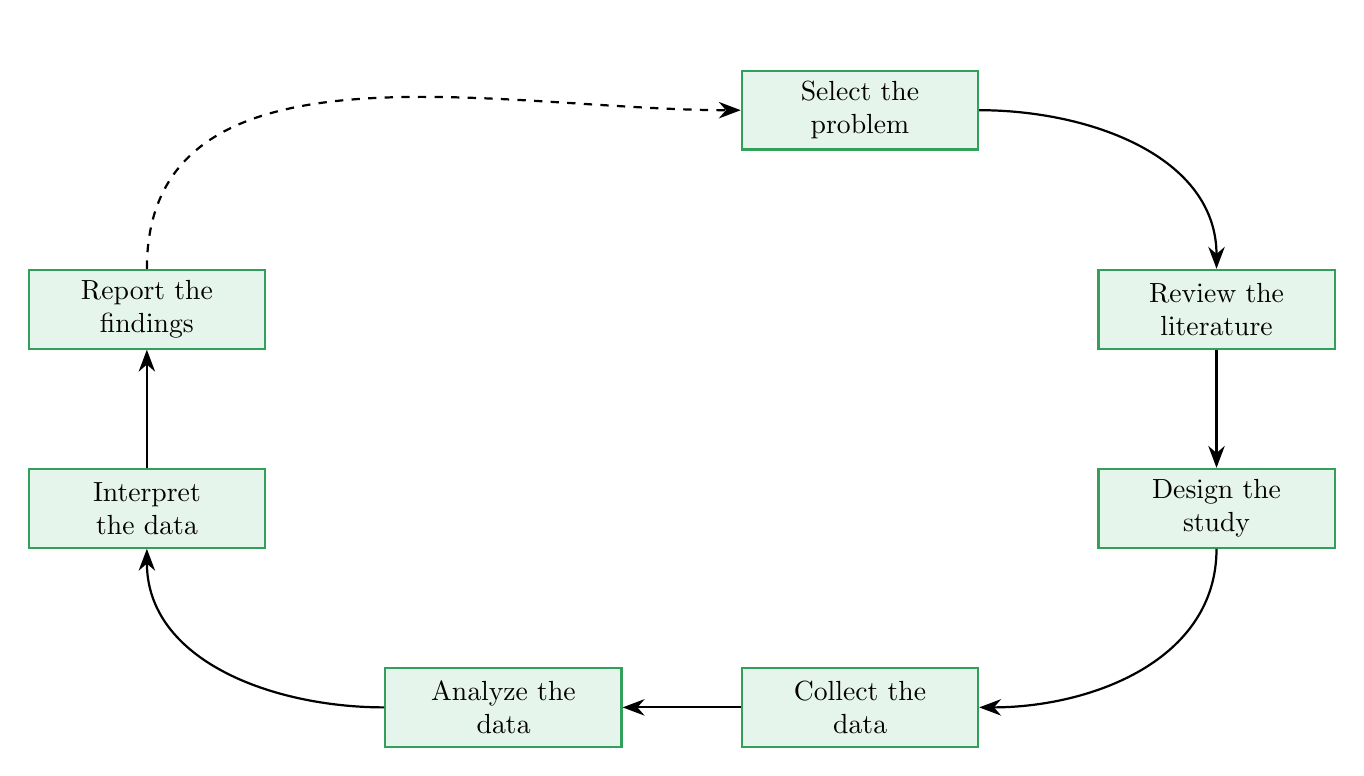
\begin{tikzpicture}[
        node distance=1.5cm and 1cm,
        box/.style={draw, rectangle, minimum width=3cm, minimum height=1cm, align=center, fill=tipbg, draw=tipframe, thick},
        arr/.style={-{Stealth[scale=1.2]}, thick}
    ]
    
    % Nodes
    \node[box] (select) {Select the\\problem};
    \node[box] (review) [below right=1.5cm and 1.5cm of select] {Review the\\literature};
    \node[box] (design) [below=1.5cm of review] {Design the\\study};
    \node[box] (collect) [below left=1.5cm and 1.5cm of design] {Collect the\\data};
    \node[box] (analyze) [left=1.5cm of collect] {Analyze the\\data};
    \node[box] (interpret) [above left=1.5cm and 1.5cm of analyze] {Interpret\\the data};
    \node[box] (report) [above=1.5cm of interpret] {Report the\\findings};

    % Arrows
    \draw[arr] (select) to[out=0,in=90, looseness=1] (review);
    \draw[arr] (review) -- (design);
    \draw[arr] (design) to[out=270,in=0, looseness=1] (collect);
    \draw[arr] (collect) -- (analyze);
    \draw[arr] (analyze) to[out=180,in=270, looseness=1] (interpret);
    \draw[arr] (interpret) -- (report);
    
    % Cycle back arrow
    \draw[arr, dashed] (report) to[out=90,in=180, looseness=1] (select);

    \end{tikzpicture}
    \caption{Siklus Berkelanjutan Tahapan Penelitian}
\end{figure}

Pecahan detail dari tiap tahapannya:
\begin{enumerate}
    \item \textbf{Menentukan Masalah:} Nyari masalah yang belum ada jawabannya, dan diubah jadi pertanyaan penelitian yang menghubungkan antar variabel.
    \item \textbf{Mengaji Pustaka:} Baca-baca literatur biar dapet wawasan yang kuat dan mastiin kita nggak ngulangin hal yang udah pernah diteliti orang.
    \item \textbf{Mendesain Penelitian:} Bikin \textit{blueprint} alias rencana strategi eksekusi buat ngejawab masalah tadi.
    \item \textbf{Mengumpulkan Data:} Turun lapangan pakai instrumen (tes, kuesioner, wawancara, dsb).
    \item \textbf{Menganalisis Data:} Ngolah data mentah tadi pakai teknik statistik yang pas.
    \item \textbf{Menafsirkan Data (Interpret):} Nyari arti dari hasil hitungan analisis. Bikin kesimpulan apakah peluang temuan kita ini valid, dan bagaimana nasib hipotesis kita (ditolak/diterima).
    \item \textbf{Melaporkan Hasil (Report):} Bikin publikasi biar ilmu pengetahuannya nambah dan siklusnya bisa dimulai lagi sama peneliti lain!
\end{enumerate}

\end{document}